%
% Appendix 2
%

\chapter{Boosted Decision Trees}
\label{app:bdts}
Boosted Decision Trees are the single MVA/machine learning technique used for discriminating signal from background
in this analysis. BDTs are used in this analysis exclusively for classification.
BDTs are a special instance of a decision tree, which is illustrated below in Figure~\ref{fig:dec_tree}.
This analysis uses the BDT implementation in the Toolkit for Multivariate Analysis (TMVA) software~\cite{tmva}, based on the
C4.5 algorithm~\cite{C4.5}.
The choice of BDTs over other MVA methods such as artificial neural networks (aNNs) or support vector machines (SVMs) is motivated
by several factors. While the cut-based classification technique the BDT relies on is a theoretically less powerful classifier compared
to other more sophisticated MVAs such as aNNs, it typically offers the best ``out-of-the-box'' performance, requiring the least amount
of optimization to acheive near-maximum performance. This simiplicity also translates to faster training and evaluation times.
Additionally, BDTs are often more robust against over-training\footnote{Over-training, or ``over-fitting'' describes the loss of generalization (as well as performance)
between the training and testing/evaluation samples. Over-training occurs when the MVA learns statistical features of the training sets that are not present in
the testing/evaluation set.}. This practically translates to using more input variables, and/or smaller training samples than more sophisticated MVAs.
The conceptual description of BDT training is described in the following sections. 
 
\begin{figure}[hbtp]
 \begin{center}
   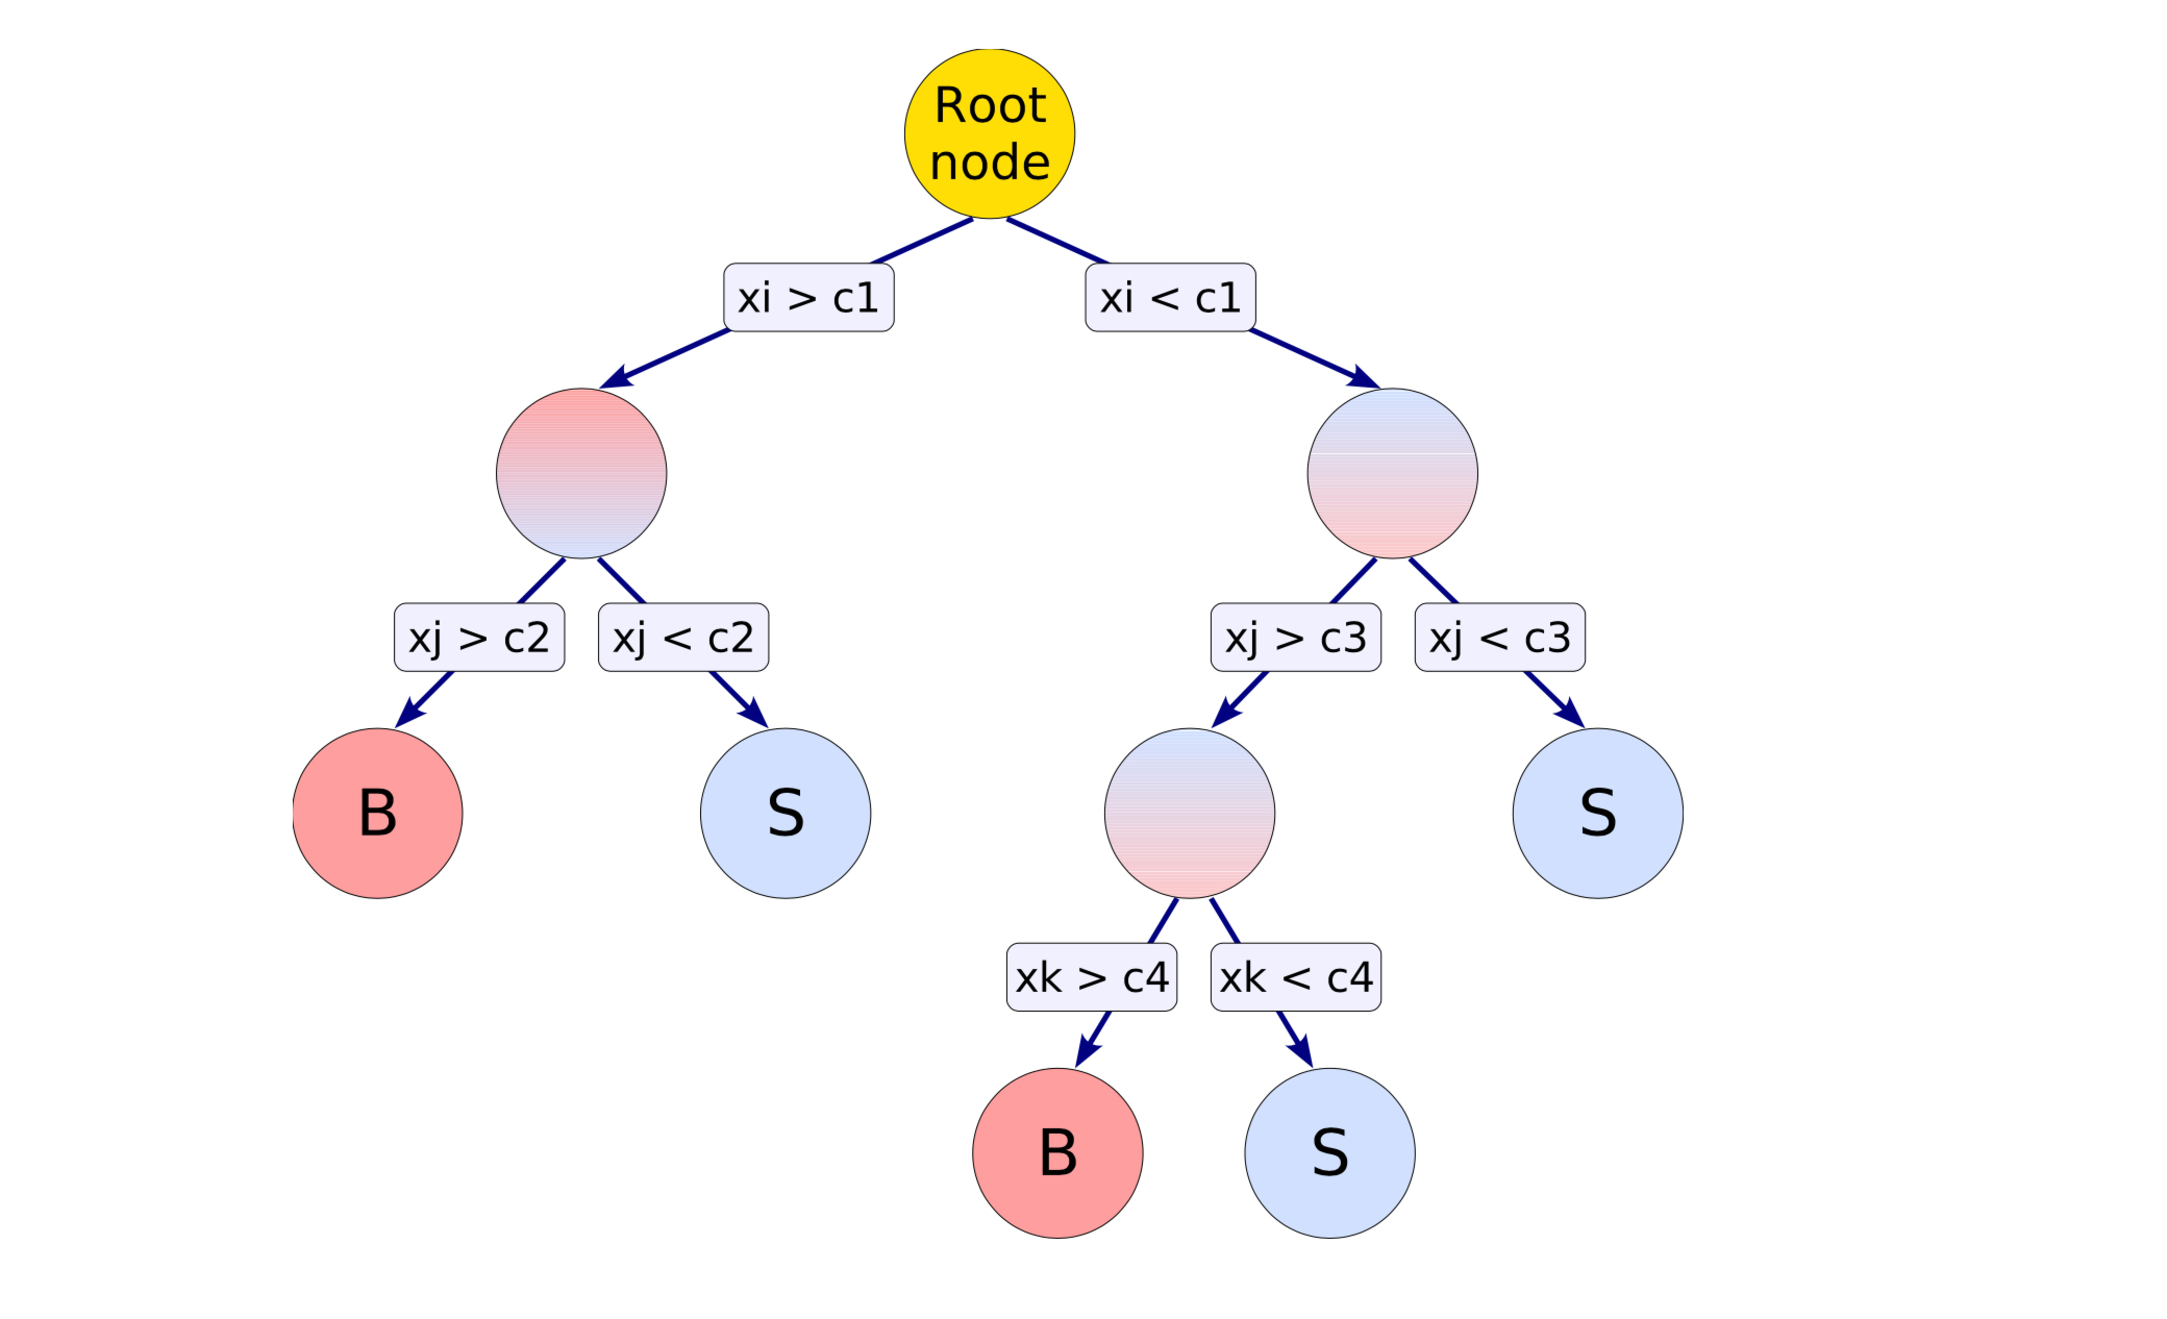
\includegraphics[width=0.8\textwidth]{ap2_figs/decision_tree.pdf}
   \caption[A decision tree diagram.]{An overview diagram of a single decision tree. The decision nodes are a mixture of red and blue,
     while the terminal nodes or leaves, are ideally depicted colored red or blue and labeled S or B for signal or background respectively~\cite{tmva}.}
   \label{fig:dec_tree}
 \end{center}
\end{figure}

\section{Tree Growth}
The decision tree begins at the root node with a single decision, or split. Given a set of inputs {$x$}, the input $x_{i}$, and the specific cut value $c_{1}$,
is selected based on best separation power between signal and background. The training events are then filtered through this first split, where events
with $x_{i} > c_{1}$ moving to the left forming a new decision node, and events with $x_{i} < c_{1}$ moving to the right, forming a new and separate 
decision node, as seen in Figure~\ref{dec_tree}. This processes is then repeated on the subsets of events in each of the two new nodes, and continued until
a specified stopping criteria is satisfied. This stopping criteria is often defined to be when a given split produces a node with purely signal or purely
background events, as illustrated in Figure~\ref{fig:dec_tree}. The stopping criteria consists of:
\begin{itemize}
\item Perfect classication
\item Not satisfying a specified minimum number of events (or fraction) of the training sample in the leaf
\item Insufficient improvement for available splittings
\item Reaching a specified maximum tree depth
\end{itemize}

One important detail not mentioned thus far is the metric used to determine ``best'' separation power when determining which variable and corresponding value to split on.
The first variable to consider for splitting criteria is purity of each node, defined as $p_{s}=\frac{s}{s+b}$, where $s$ and $b$ correspond to the number of signal and background
events in the node respectively. $p_{s}$ is 1 for a node with pure signal, and zero for a node with pure background. A $p{s}$ of 0.5 corresponds to equal amounts of signal and background
in the node. With a definition of purity, we define a figure of merit (FOM) called \textit{impurity}. The impurity of a given node $t$, is based on the purity and is denoted as
$\phi(t)$.
The impurity of a given node is maximized when the two classes (signal, background) are mixed in equal proportion $\phi(t) = 1/2$. The impurity is minimized when the node is pure
signal or pure background where $\phi(t) = 0$.
It makes more sense to work with the weighted impurities however, where a given node impurity is weighted by the number of events in that node. This quantity
will be referred to as weighted impurity $I(t) = \phi(t)N_{t}$, where $N_{t}$ is the number of events in the node. 
The splitting criteron maximizes the impurity gain, $\DeltaI(t)$. For a given node $t_{0}$ with $N_{0}$ events, we want to
select the best variable and value to split into two child nodes, $t_{L}$, with $N_{L}$ events, and $t_{R}$,with $N_{R}$ events, where $N_{0} = N_{L} + N_{R}$. Here, the
impurity gain for a given split is $\DeltaI(t) = I(t_{0}) - I(t_{L} - I(t_{R}))$, and we choose the cut which maximizes $\DeltaI(t)$ over all possible splits for all variables.
The functional form of $\phi(t)$ has not been given since there are a number of options. The simplest form of $\phi$ is the training error $\epsilon(t) = min(p_{s},p_{b})$.
The training error as the basis for the FOM suffers fro. To illustrate this shortcoming, see Figure~\ref{fig:tree_split}. Both splits produce
the same training error (25$\%$), however the split on the right is clearly a more powerful separator. Other forms of $\phi$ that avoid this scenario by punishing
event mis-classifications non-linearly include the Gini index $\phi = 1 - p_{s}^{2} - p_{b}^{2}$, and the cross entropy $\phi = \frac{-p_{s}log(p_{s})+p_{b}log(p_{b})}{2}$.
The FOM used for the BDTs in this analysis is the Gini index, which punishes mis-classifications less severely for more equal distributions of signal and background, and more
severely for mis-classifications of very unequal distributions of signal and background in a node. This is demonstrated in Figure~\ref{fig:misclass_plot}.

\begin{figure}[hbtp]
 \begin{center}
   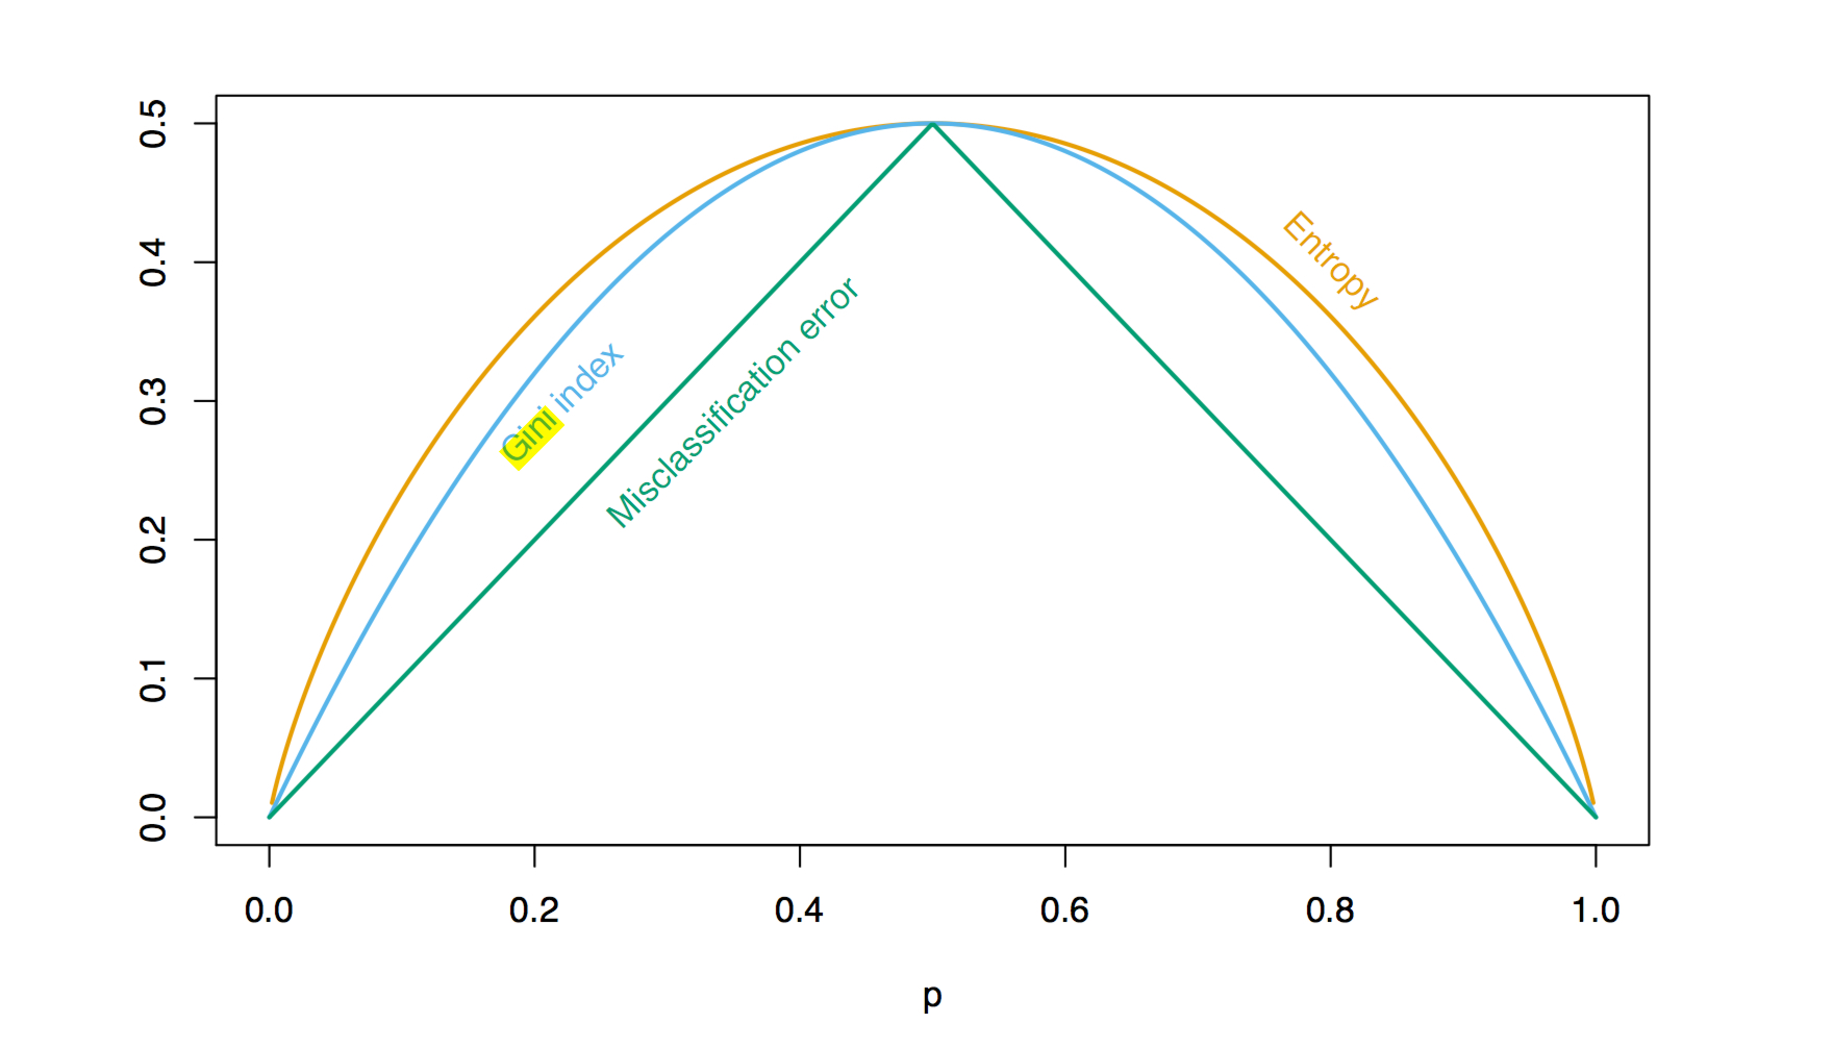
\includegraphics[width=0.8\textwidth]{ap2_figs/misclass_plot.pdf}
   \caption[Plot of misclassifcation impurity functions.]{The impurity functions vs the signal purity~\cite{esii}.}
   \label{fig:misclass_plot}
 \end{center}
\end{figure}


\section{Boosting}
The boosting method used in this analysis is the stochastic gradient boost, a form a gradient descent optimization for decision trees. Thus far the process begins with a single
weak classifier (a single tree). The training set will be comprised of events with {${$x$}_1$,$y_{1}$}....{${$x$}_N$,$y_{N}$} for N events. {$x$}$_{i}$, $y_{i} \in [0,1]$
are the input variables and class (background, signal) for event $i$. An implicit assumption in MVA training is that there exists
some function $F'(x)$, that maps a set of inputs to the event's class $y$, that is $F'(x) = y$. In training we are attempting to model this function empirically. 

The first step in gradient boosting is to grow a single tree. This single tree is $F(x)$. Surely $F(x_{i}) \neq y_{i}$ for most events, but perhaps $F(x_{i}) \approx y_{i}$
for some events. We now grow a second tree $h(x)$, such that $F(x) + h(x) = y$.

\section{Pruning}
Once the tree has been grown, it is ``pruned'' where leaf nodes are removed. This process is also referred to as tree regularization. 

